\documentclass[UTF-8]{ctexbeamer}
\usetheme{Copenhagen}
\usecolortheme{seahorse}

\usepackage{multimedia}
\usepackage{listings}
\usepackage{minted}
\usepackage{tikz}
\usepackage{textcomp}
\usepackage[normalem]{ulem}

\title{Something Something Memory Ordering}

\author{喵喵}
\date{2022.1}

\begin{document}
\begin{frame}
  \titlepage
  \begin{center}
    
\includegraphics[width=.1\textwidth]{assets/float.png}
  \end{center}
\end{frame}

\begin{frame}
  \frametitle{Somewhere on the Internet...\footnote{\url{https://lwn.net/ml/linux-kernel/CAHk-\%3DwgJZVjdZYO7iNb0hFz-iynrEBcxNcT8\_u317J0-nzv59w\%40mail.gmail.com/}}}

  \begin{block}{Wed, 09 Jun 2021 11:25:24 -0700}
...

\vspace{1em}

Look, memory ordering pretty much \_is\_ the rocket science of CS, but
the C standards committee basically made it a ton harder by specifying
"we have to make the rocket out of duct tape and bricks, and only use
liquid hydrogen as a propellant".

\vspace{1em}

\pause

Linus
  \end{block}
\end{frame}

\begin{frame}[fragile]
  \frametitle{What}

  你要写个锁:

  \begin{minted}{c}
  bool locked;

  // Aquire lock
  while(atomic_swap(locked, true)) cpu_yield();

  // Critical section
  feed_cats()

  // Release lock
  locked = false;
  \end{minted}
\end{frame}

\begin{frame}
  \frametitle{What}

  O3 万事皆有可能!
  \pause

  {
    \tiny
  其实不 O3 也有可能!
  }

\end{frame}

\begin{frame}
  \frametitle{Why}

  \pause

  Decades-long 内卷 in $\mathrm{\mu}$Arch

  \pause
  General theme: 隐藏延迟

  \pause
  但是延迟并未消失,会在 Least expect 的时候影响程序行为。

  \pause
  \vspace{1em}

  TL;DR: 因为\textbf{缓存层级}、\textbf{多核心}以及\textbf{乱序执行}互相背刺的结果
\end{frame}

\begin{frame}
  \frametitle{Cache Hierarchy}
  延迟 vs. 面积 vs. 吞吐量
  
  \vspace{1em}

  \pause

  多计算核心会导致问题:缓存不一致
\end{frame}

\begin{frame}
  \frametitle{Coherence Protocol}
  一般的实现:MESI 协议
  \pause
  \begin{itemize}
    \item Modified: 本地存储有更改后的内容,兄弟节点不能拥有有效的这块儿数据
    \item Exclusive: 本地是唯一一份兄弟节点中有效数据
    \item Shared: 本地和兄弟节点共享这份数据
    \item Invalid: 本地没有这份数据
  \end{itemize}
  \pause
  \vspace{1em}
  需要某种方式传递 Coherence 信息
  \pause
  \begin{itemize}
    \item Snooping: 一个 Coherence bus
    \item Directory: 一个 Coherence master
  \end{itemize}
\end{frame}

\begin{frame}
  \frametitle{Interconnect}

  Problem: interconnect 有\only<2->{\textbf{不稳定的}}延迟
  
  \pause
  \pause
  \vspace{1em}

  不同的 Coherence 信息可能在 Interconnect 网络内花不同的时间传递!

  \pause
  e.g. NUMA, distributed LLC, ...

  \pause

  为了维持更强的内存序,需要牺牲 Interconnect / NoC 的性能保序。
\end{frame}

\begin{frame}[fragile]
  \frametitle{E.g.}
  \begin{block}{Core A}
    \begin{minted}{c++}
// Initially, *ptrA == *ptrB == false
*ptrA = true;
*ptrB = true;
    \end{minted}
  \end{block}
  \begin{block}{Core B}
    \begin{minted}{c++}
int readA = *ptrA;
int readB = *ptrB;
assert(!(readA == false && readB == true));
    \end{minted}
  \end{block}

  \pause

  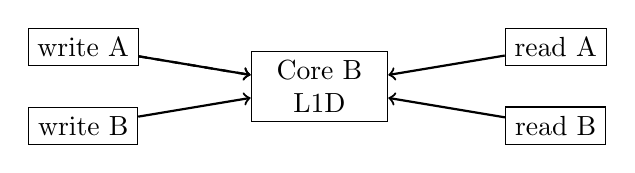
\begin{tikzpicture}
    \node (wB) at (0, 0) [draw] {write B};
    \node (wA) at (0, 1) [draw] {write A};

    \node (rB) at (6, 0) [draw] {read B};
    \node (rA) at (6, 1) [draw] {read A};

    \node (core) at (3, 0.5) [draw,text width=1.5cm,align=center] {Core B \\ L1D};

    \draw[->,thick,dashed] (wA) edge (core);
    \pause
    \draw[->,thick] (wB) edge (core);
    \pause
    \draw[->,thick] (rA) edge (core);
    \draw[->,thick] (rB) edge (core);
    \pause
    \draw[->,thick] (wA) edge (core);
  \end{tikzpicture}
\end{frame}

\begin{frame}[fragile]
  \frametitle{E.g. 2}
  \begin{block}{Core A}
    \begin{minted}{c++}
*start = true;
    \end{minted}
  \end{block}
  \begin{block}{Core B}
    \begin{minted}{c++}
while(!*start) // spin;
*end = true;
    \end{minted}
  \end{block}
  \begin{block}{Core C}
    \begin{minted}{c++}
while(!*end) // spin;
assert(*start)
    \end{minted}
  \end{block}
\end{frame}

\begin{frame}[fragile]
  \frametitle{E.g. 3}
  \begin{columns}

    \begin{column}{0.5\textwidth}
      \begin{block}{Core A}
        \begin{minted}{c++}
*ptrA = true;
        \end{minted}
      \end{block}
      \begin{block}{Core C}
        \begin{minted}{c++}
while(!*ptrA) ;
while(!*ptrB) ;
*cnt += 1;
        \end{minted}
      \end{block}
    \end{column}

    \begin{column}{0.5\textwidth}
      \begin{block}{Core B}
        \begin{minted}{c++}
*ptrB = true;
        \end{minted}
      \end{block}
      \begin{block}{Core D}
        \begin{minted}{c++}
while(!*ptrB) ;
while(!*ptrA) ;
*cnt += 1;
        \end{minted}
      \end{block}
    \end{column}

  \end{columns}
\end{frame}

\begin{frame}
  \frametitle{Also be careful for...}

  \begin{itemize}
    \item Store buffers
    \item Victim FIFO
  \end{itemize}
\end{frame}

\begin{frame}
  \frametitle{Out-of-Order Pipeline}

  Welcome to the mess\textsuperscript{TM}.
  \pause
  现在L1D看到的访存和真正的访存顺序都可以不一样了!

  \pause
  \vspace{1em}

  一个常见优化:非阻塞缓存——允许后发生的,没有 Miss 的访存请求先返回。
\end{frame}

\begin{frame}
  \frametitle{What's the cost...}
  为了\sout{追逐力量}进行微架构优化,我们使得:

  \begin{itemize}
    \item 访存指令发射的顺序可能和真实顺序不同
    \item L1D 处理访存的顺序可能和指令发射的顺序不同
    \item 其他节点接收到 Coherence 消息的顺序可能和发出的顺序不同,或者不一致
  \end{itemize}
\end{frame}

\begin{frame}
  \frametitle{To regain sanity...}
  定义 Memory order: 一些访存操作的额外属性,约束编译器和微架构实现的优化。

  \pause
  \vspace{1em}

  \begin{itemize}
    \item Sequence Consistent:要求所有带有这一属性的访存在全局有一个一致的观测顺序。
    \item Acquire-Release 语义:对应常见的锁的实现
    \begin{itemize}
      \item Acquire: (通常作为读取)其后的访存不允许重排到其之前。
      \item Release: (通常作为写入)其前的访存不允许重排到其之后。
    \end{itemize}
    \item Relaxed: 代表没有任何额外要求
  \end{itemize}

  \pause
  \vspace{1em}

  通常为了保证软件不需要滥用这些访存约束,ISA 通常会给出额外的一些约束,放弃不重要的优化,使得常见的访存模式可以给出符合直觉的结果。

  \pause
  e.g.: 要求同一个核心的 RAW 访问符合直觉。
\end{frame}

\begin{frame}
  \frametitle{Case: RVWMO \& Tilelink \& BOOM}
  \pause
  \sout{我很想讲 BOOM 但我不太会,GG}
\end{frame}

\begin{frame}[fragile]
  \frametitle{Case: RVWMO \& Tilelink \& BOOM (疑似)}

  RVWMO TL;DR:
  \begin{itemize}
    \item 默认核心内部 Strong order, 核心之间 Weak order
    \begin{itemize}
      \item 额外的,不允许 L-L 重排
    \end{itemize}
    \item Acquire-Release 语义 + Sequential consisten 要求
    \item LL/SC + AMO
  \end{itemize}

  \begin{block}{L-L 重排}
    \begin{minted}{asm}
      ld a0, 0(s0)
      ld a1, 0(s0)
      // a0 NOT ALLOWED to get newer versions than a1
    \end{minted}
  \end{block}
\end{frame}

\begin{frame}
  \frametitle{Case: RVWMO \& Tilelink \& BOOM (疑似)}

  Tilelink TL;DR:
  \begin{itemize}
    \item 节点拓扑构成有向无环,单一路径的图,方便维护 Coherence 状态。节点需要维护孩子的 Coherence 状态。
    \item 经典的 MESI + 扩展(见下图)
    \item 典型实现中,AMO 操作在 Coherence master (LLC) 处发生
  \end{itemize}

  \begin{figure}
    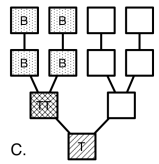
\includegraphics{assets/tilelink.png}
    \caption{TileLink 节点 Coherence 状态}
  \end{figure}
\end{frame}

\begin{frame}
  \frametitle{Case: RVWMO \& Tilelink \& BOOM (疑似)}

  Tilelink 这样的设计允许的优化 e.g.:
  \begin{itemize}
    \item 对应 RVWMO,对核心和缓存的实现比较方便
    \item 修改的版本存储在最接近访问的地方,减少 Writeback 所用的带宽
    \item 用于同步的内存访问发生在 LLC,减少 Coherence message 所用的带宽
  \end{itemize}

  \pause

  禁止的优化 e.g.:
  \begin{itemize}
    \item 不允许多条路径,因此无法实现 Distributed L2 / LLC
  \end{itemize}
\end{frame}

\begin{frame}
  \frametitle{Case: RVWMO \& Tilelink \& BOOM (疑似)}

  BOOM (疑似) TL;DR:
  \begin{itemize}
    \item 是一个乱序处理器!积极发射所有的访存,遇到违反核心内部顺序或者 L-L 重排时发送微架构异常刷新流水线。
    \item 非阻塞 Cache
  \end{itemize}

  \vspace{1em}
  \pause
  如果允许更弱的内存序,可以实现更多优化:
  \begin{itemize}
    \item 允许核心内访存重排:完全不检查任何访存乱序
  \end{itemize}
\end{frame}

\begin{frame}
  \frametitle{Other Considerations}

  \begin{itemize}
    \item Speculative execution
    \item Prefetch
    \item I\$ Coherence?
    \item Non-explicit memory access (page table, A/D bits)
  \end{itemize}
\end{frame}

\begin{frame}
  \frametitle{RISC-V ISA 的其他相关细节}

  允许的优化:
  \begin{itemize}
    \item 显式 FENCE.I / SFENCE.VMA,不需要 Coherence I\$ / TLB
    \item PMA 只有部分内存需要支持 AMO (对应 TileLink 的特定 Message)
  \end{itemize}

  导致的实现要求
  \begin{itemize}
    \item 页表访问遵循 RVWMO,直接导致所有的实现基本都将 PTW 连接到 D\$ 上
  \end{itemize}
\end{frame}

\begin{frame}
  \frametitle{That's All!}

  \begin{center}

    
\includegraphics[width=.5\textwidth]{assets/look.png}

    Question time!
  \end{center}
\end{frame}
\end{document}
